% TODO: rework architecture to talk more about NetCheck
% TODO: Verify information on supported trace formats

\section{CrashSimulator Approach Details}

    \begin{figure}[h]
        \center{}
        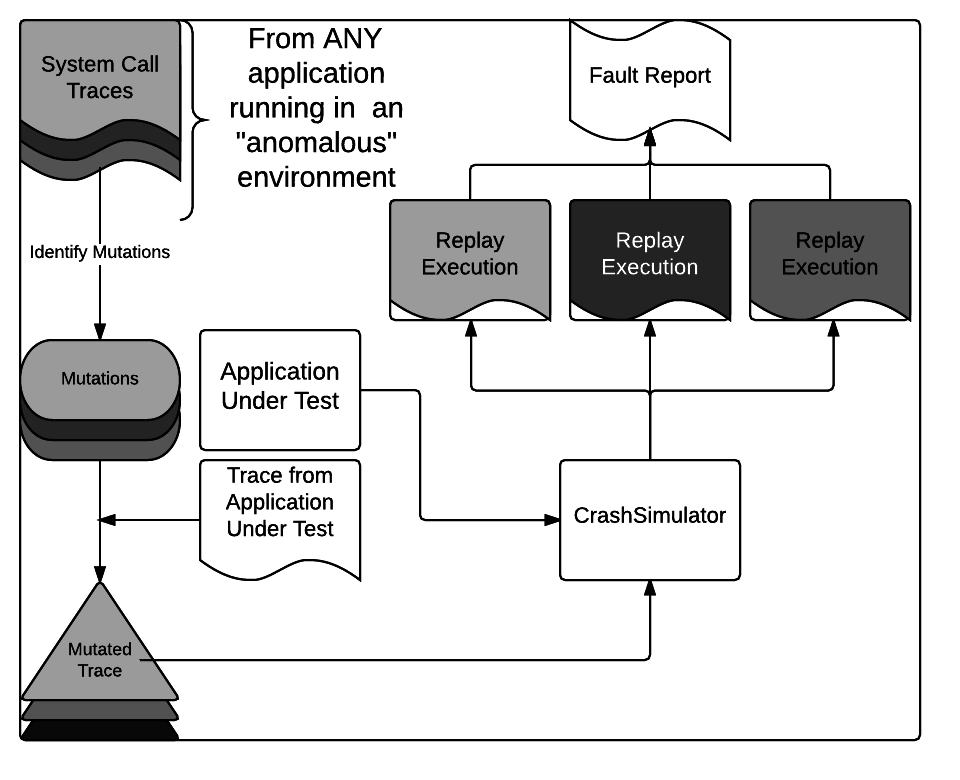
\includegraphics[scale=.5]{Architecture}
    \end{figure}

    \subsection{Architecture}

        At a high level CrashSimulator is organized into three primary modules. First, there is the system call trace
        parser. This module is responsible for interpreting the input system call traces and identifying opportunities
        to inject faults into the application under test. Second, there is the test control module. This module is
        responsible for iterating through the list of potential anomalies generated by the system call trace parser and
        in order to test each one of them. Finally, there is the test launcher. This module is responsible for launching
        the application under test and performing the interactions necessary to inject the test fault and monitor the
        application's response.

        CrashSimulator was designed this was in order to maximize code reuse and portability. A great deal of work has
        already been accomplished by NetCheck and CheckAPI in the domain of system call trace parsing. \emph{Strace} and
        \emph{dtrace} both produce output that was primarily intended for human rather than programmatic consumption. As
        such, reuse of their parsing code resulted in a large time savings and increased confidence in parsing accuracy.

        % TODO: More Detail!!!
        During parsing CrashSimulator makes use of a group of supported strategies. These strategies along with
        configurable rule sets are used to identify ``interesting'' system calls into which faults will be injected
        during the testing phase. The output from this module is a ``test plan'' that contains a list of tests to be run
        by the test controller. A test consists of the system calls to be modified and the modification to make.

        The test launcher was separated from the test controller for the sake of portability. A great deal of the test
        launcher's code deals with the low level details of process manipulation and monitoring and, as such, will
        likely require modification in order to operate on different platforms than the authors' original development
        environments. For example, in order to modify the return value of particular system calls on x86 systems, the
        test launcher must hook the application under test using \emph{ptrace} and modify the values of the EAX register
        upon completion of the system call. This modification is tightly coupled to x86 calling conventions. Even the
        relatively similar x86--64 differs in that the test launcher must use \emph{ptrace} to modify the RAX register
        rather than the EAX register. Other architectures, such as ARM, will likely require more extensive
        modifications.

        All three primary CrashSimulator modules are packaged together and interact with each other at the appropriate
        times without user intervention. At this point, CrashSimulator itself is available as a virtual machine
        appliance compatible with the \emph{Virtual Box} virtual machine hosting software. The reasons for distributing
        CrashSimulator in this manner are threefold. First, this distribution method ensures that all of
        CrashSimulator's dependences are installed and configured appropriately. Second, this method provides an
        environment for taking system call traces that is known to be complete tool-wise and compatible with
        CrashSimulator. Finally, and most importantly, this method provides an environment that is known to be
        compatible with the low level details of CrashSimulator's fault injection techniques.

        CrashSimulator's source code is available and, while other environments may be untested, it should function
        correctly on any platforms that meet the criteria described above.

    \subsection{System Call Traces}

        The first step in CrashSimulator's operation is to gather a trace of the system calls made by the application
        during a normal run. Where other tools base their operation of direct analysis of the application under test
        CrashSimulator operates based on information gleaned from system call traces. This gives CrashSimulator several
        advantages over similar tools. First, CrashSimulator operates in a language independent manner. It can test any
        program given two conditions hold true:

        \begin{enumerate}
            \item{The application can run in the testing environment}
            \item{The testing environment has the tools required to take a system call trace of the application during
            a normal run}
        \end{enumerate}

        This removes the need for the complex language parsing that other similar tools rely on. Second, the faults
        injected by CrashSimulator test the interface between the application under test and its environment. Other
        similar testing tools focus on testing the logic within the application under test which missing faults that
        only appear when the application is run in an imperfect, real world environment.

        Because CrashSimulator's trace analysis engine is based on prior work from the NetCheck supported trace
        gathering tools include \emph{strace} on Linux and \emph{dtrace} on OS X.

    \subsection{Identifying Injection Points}

        CrashSimulator has three strategies for identifying a section of a system call trace as an interesting point for
        fault injection. There is a many-to-many relationship between the strategies described here and the fault types
        that can be injected that are discussed later in this section.

        % TODO: More Detail!!!
        \subsubsection{Pattern Matching}

            This injection point identification strategy is the most straightforward in description and implementation.
            CrashSimulator simply searches through the system call trace line-by-line identifying all system calls that
            match a rule in CrashSimulator's pattern matching rule set. For example of rule that results in a ``return
            value modification'' injection could be as follows: Match a call to the \emph{connect} system call that was
            successful (i.e.\ the system call returns 0) and modify the return value to be -1 (i.e.\ failure) during a
            subsequent test run. This strategy generates a single test for each line in the system call trace that
            matches a rule.

            This strategy has two main advantages. First, it is relatively simple to implement and processing the system
            call traces in this manner is fairly inexpensive computationally. At the same time, this strategy produces a
            very large number of tests and an extensive rule set can provide a high degree of system call coverage.

        % TODO: More Detail!!!
        % TODO: Rename to group based? Or something similar?
        \subsubsection{Catalog Based}

            This injection point identification strategy is a step up in complexity from the Pattern Matching strategy
            and as a result it is able to generate tests that catch faults at a slightly higher level of abstraction.
            With this strategy, a set of system calls is identified in a rule set and they are analyzed collectively.
            This allows for modifications across a whole group of system calls at the same time. For example, a
            simplistic case might be modifying the return values of all of a set of system calls at the same time. A
            more complex case would be reordering the data returned by all recvfrom system calls to replicate out of
            order receipt of UDP datagrams.  In this strategy, each rule generates a single test that modifies a group
            of system calls.

        % TODO: More Detail!!!
        \subsubsection{Condition Based}

            This injection point identification strategy is the most complex offered by CrashSimulator. Rules for this
            strategy allow for the identification of system calls based on the success or failure of previous system
            calls.  Rules are specified in the form of an ordered list of system calls and their expected return values.
            A match occurs when the final system call in the list is reached and the prior system calls occurred in
            order with the appropriate return values. An example would be modifying a subsequent call to recv to fail
            only if the prior call to recv was successful.

    \subsection{Potential Deviations}

        \textbf{I would really like to find another term besides anomaly}

        CrashSimulator's goal when analyzing a normal run system call trace is to identify individual system calls or
        patterns of system calls that it recognizes as an opportunity to inject a fault during subsequent runs. These
        signatures are referred to as ``potential anomalies.'' CrashSimulator has the ability to identify and classify
        anomalies into the following categories.

        \subsubsection{Return Value Modification}

            One way CrashSimulator can inject faults into the running application is to modify the return values of
            interesting system calls identified in the previous trace analysis step. The primary driver behind injecting
            this type of fault is the tendency of developers to misuse common API functions or misunderstand their
            failure modes. The \emph{recv} system call, for example, returns the number of bytes of data it was able to
            copy into the requested buffer from the specified socket. A developer that is unfamiliar with the operation
            of \emph{recv} may assume that a positive return value means that \textbf{all} of the requested data was
            successfully copied. This assumption fails to account for cases where the system call completed successfully
            but copied less data than the developer was expecting. A well written application might make repeated calls
            to recv until it has gathered all the data it needs while an incorrectly written application may only call
            it once resulting in a fault when it tries to process incomplete data in the future.

            % TODO: Make sure terminology is correct in this paragraph
            % TODO: Is this methodology reasonable?
            The authors' implementation of CrashSimulator injects this fault using ptrace. The application under test is
            executed in a process that is hooked by ptrace and each system call made by the application is examined.
            When a system call that was previously identified as a target is encountered execution interrupted
            immediately upon its completion. At this point the return value of the system call is modified using rules
            defined on a per system call basis. These rules are based on the system calls normal operation and return
            values. For example, if a recv call is identified as interesting and returns a positive value (i.e.\ success)
            in the normal system call trace, this same call would be modified to return -1 (i.e.\ error) during a test
            run. Other modifications would include changing the positive return value to 0 and to some other positive
            number that is less than the original return value.

            Should modification of return value depend on the value from the initial run or the value returned during
            the test???

            % TODO: Rework the example described here
        \subsubsection{Data Reordering}

        \emph{I need to write these bullet points up in paragraph form}
        \begin{itemize}
            \item{supported by catalog based}
            \item{identify group of system calls in question}
            \item{hand in re-ordered data from ideal run}
            \item{dependent on data collected in the ideal run}
        \end{itemize}


            First, the normal run trace is parsed in its entirety for system calls in a specific set
            associated with the fault being injected and the data items passed into these system calls are recorded in a
            data item catalog. Next, the application under test is run repeatedly with each run receiving a different
            ordering of data items from the catalog for the corresponding system calls. One example of a fault
            CrashSimulator can inject in such situations is unhandled out of order UDP datagrams. Consider the following
            pseudo-code listing:

            % TODO: Use the real C Code here
            \begin{verbatim}
int main() {
    socket = setupUdpSocket()
    data1 = recvfrom(socket)
    processData1(data1)
    data2 = recvfrom(socket)
    processData2(data2)
}
            \end{verbatim}

            This listing sets up a UDP socket and receives two datagrams from the socket processing each with the
            appropriate function. A C program that implements this pseudo-code will produce a normal flow system call trace
            as follows:

            %\begin{verbatim}
% ...
% socket(PF_INET, SOCK_DGRAM, IPPROTO_UDP) = 3
% bind(3, {sa_family=AF_INET, sin_port=htons(6666), sin_addr=inet_addr("0.0.0.0")}, 16) = 0
% recvfrom(3, "test\n", 256, 0, {sa_family=AF_INET, sin_port=htons(51490), sin_addr=inet_addr("127.0.0.1")}, [16]) = 5
% ...
% write(1, "Process 1: test\n", 16)       = 16
% recvfrom(3, "testagain\n", 256, 0, {sa_family=AF_INET, sin_port=htons(51490), sin_addr=inet_addr("127.0.0.1")}, [16]) = 10
% write(1, "Process 2: testagain\n", 21)  = 21
% ...
            %\end{verbatim}
            \textbf{\emph{Sample trace removed}}
            The above program assumes that datagram 1 will always arrive first and datagram 2 will always arrive second. UDP
            makes no ordering guarantees so the reverse is possible. This would result in datagram 2 being processed as
            datagram 1 and vice versa. Crash simulator would inject this fault as follows. First, it would parse the system
            call trace and identify all calls to recvfrom, storing the data that was received in a data catalog and the
            identifying information pertaining to the socket it was received from. Second, it would re-run the application
            under test and send a different ordering of data from the data catalog to the socket in question. From the above
            example, ``testagain'' would be sent to the first receive from and ``test'' would be sent to the second recvfrom
            resulting in each data item being parsed by the incorrect function. CrashSimulator would then report
            abnormalities in the application's behavior. \textbf{How are we going to handle situations where this is a
            silent failure}

        \subsubsection{Blind Data Modification}

            supported by pattern matching, catalog based, conditional
            Identify system call in question
            Perform modification described in test to data
            Doesn't depend on data from the ideal run
